\documentclass[11pt]{article}
\usepackage[top=0.20in, bottom=.20in, left=0.5in, right=0.5in]{geometry}
\renewcommand{\baselinestretch}{1.1}
\usepackage{graphicx}
\usepackage{natbib}
\usepackage{amsmath}
\usepackage{multicol}
\usepackage{tcolorbox}
\usepackage{caption}
\usepackage{todonotes}
\usepackage[font={sf,footnotesize}]{caption}
\usepackage{hyperref}
\newcommand{\llabel}[1]{\hypertarget{lintarget:#1}{}\linelabel{lin:#1}}

\usepackage{lineno}
\renewcommand\linenumberfont{\normalfont\tiny\color{gray}}


\bibliographystyle{besjournals}

\begin{document}

% \title{Closing the gap between statistical and scientific workflows for improved forecasts in ecology} 
\title{\large Closing the gap between statistical and scientific workflows for improved forecasts in ecology\\Supplementary material}
\date{}
\author{\small Victor Van der Meersch$^{1*}$, James Regetz$^{2}$, T. Jonathan Davies$^{1,3}$ \& EM Wolkovich$^{1}$}
\maketitle
{\footnotesize \noindent $^{1}$ Forest and Conservation Sciences, University of British Columbia, Vancouver, BC V6T 1Z4, Canada\\
$^{2}$ National Center for Ecological Analysis and Synthesis, 1021 Anacapa St, Santa Barbara, CA 93101, United States\\
$^{3}$ Botany, University of British Columbia, Vancouver, BC V6T 1Z4, Canada \\
$^{*}$ \url{mailto:victor.vandermeersch@ubc.ca}

\renewcommand{\thefigure}{S\arabic{figure}}

\begin{figure}[b]
	\centering
    \vspace*{-20cm}
	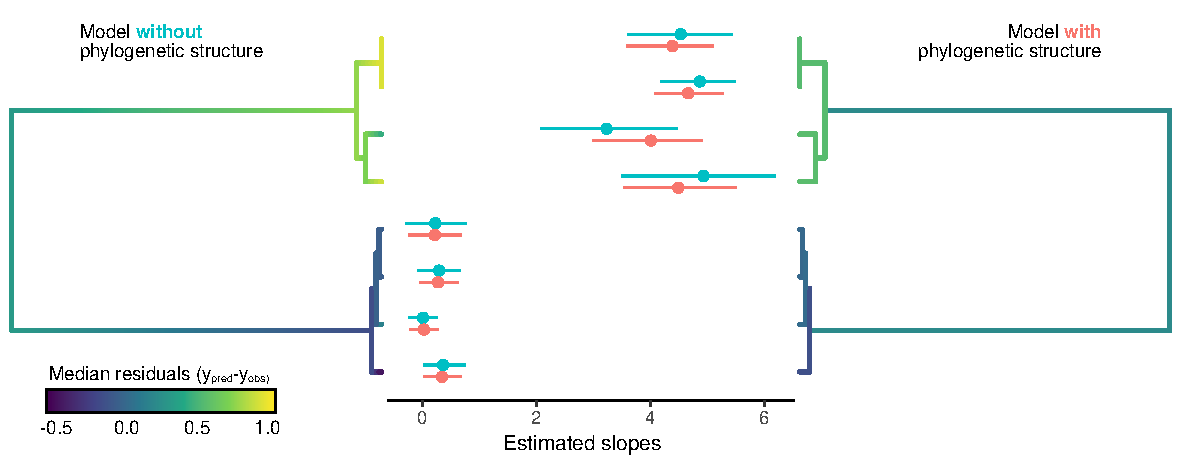
\includegraphics{../figures/retrodic/retrodictive_check_slopes.pdf}
	\caption{A simple illustration of a retrodictive check to highlight a missing structure in a model. Here, we consider ``observations'' simulated from a linear regression model ($y_\text{obs}$) for 8 different species as an example of what could happen using empirical data on time-series observations of abundance for multiple species. In this example, we simulated species-specific intercepts and slopes with a phylogenetic structure, i.e. the correlation between two species-specific parameters is proportional to the amount of evolutionary history (as defined by a simulated phylogenetic tree, shown in the left and right parts of the figure) shared by the two species. \\
	As a first approach we may often take in model-fitting of such data, we used a model with partial pooling on the intercepts and the slopes---assuming no correlation structure. We then simulated data from the fitted model ($y_\text{pred}$) and compared the retrodictions to the observations---i.e. doing a retrodictive check. The check has to be tailored in regard to our research question and our domain expertise: here, we believe that the shared evolutionary history of species could shape their responses, and thus we want to visually check whether we find any apparent differences between species groups (``clades''). In the left part of the figure, we find some (small) symptoms of a missing group structure: the upper clade residuals tend to have a positive bias, while the lower clade ones have a negative bias. This retrodictive check indicates that we could refine our model, using the phylogenetic correlation structure (in this case, because we have simulated this example, we know this structure, provided by the phylogenetic tree we used, is relevant). With this new refined model, we can perform a new retrodictive check (right part of the figure): the difference of residual biases between the two distinct clades now appears smaller. \\
	However, we do not observe an important shift in the residuals (i.e.in the $y_\text{pred}$ themselves). Rather, the addition of correlation structure in our second model mostly result in a reduction in species-specific parameter uncertainty (middle part of the figure in cyan and blue, with lines representing IQR and dots the medians).}
	\label{fig:modeldata}
	\vspace*{2cm}
\end{figure}

\end{document}
